% SC4063 --- Chapter 5: Denial-of-Service and Availability Defence (0->100)
\chapter{Denial-of-Service and Availability Defence}\label{ch:ddos}
\sloppy

\begin{quote}
\emph{``Availability is the quiet property: you notice it only when it is gone.''} --- Confidentiality and integrity hide secrets; availability keeps the door open for the honest while closing it for the flood.
\end{quote}

\noindent\fbox{\parbox{\dimexpr\linewidth-2\fboxsep-2\fboxrule}{%
\textbf{From zero: flooding a pipe until the honest cannot speak.} We start from one SYN, add ten thousand bots, then a reflector that shouts back louder than it was spoken to. Picture first (bot $\to$ amplifier $\to$ victim), then arithmetic (amplification factor), then defence (cookies, policing, scrubbing). No prior DoS background assumed.}}
\vspace{0.4em}

\section*{Learning Outcomes}
After this chapter you will be able to:
\begin{enumerate}[label=(L\arabic*)]
    \item classify DoS/DDoS as volumetric, protocol, or application-layer and give an example of each;
    \item explain botnets, reflectors, and pulsing attacks and compute an amplification factor;
    \item describe the SYN-flood backlog and how SYN cookies trade state for computation;
    \item compare rate policing, blackholing, scrubbing centres, and Anycast/CDN absorption;
    \item execute a detect$\to$classify$\to$filter$\to$scale$\to$post-mortem playbook.
\end{enumerate}

% ============================================================
\section{Taxonomy: What Does ``Down'' Mean?}\label{sec:ddos-tax}
Availability means an authorised request receives a correct response within its deadline. Denial-of-service breaks that promise by exhausting a bottleneck: bandwidth, packets-per-second, connection state, or application logic. One sender is DoS; many senders is DDoS and is strictly harder because the ingress is diffuse.

\begin{description}[leftmargin=1.2em,itemsep=0.35em]
    \item[Volumetric] Fill the pipe. UDP floods, DNS/NTP amplification, and carpet-bombing saturate links or PPS budgets. Defence is absorbing or diverting bits elsewhere (Anycast, CDN, scrubbing). Rate limits near the victim help little because the link before the filter is already full.
    \item[Protocol] Abuse the handshake, not the payload. SYN flood leaves half-open state,fragment floods exhaust reassembly, and Slowloris holds application slots with partial headers. Defence is making state cheap or stateless (SYN cookies, timeouts) and policing per-source.
    \item[Application] Look legitimate but cost dearly. HTTP GET floods, expensive API calls, and TLS renegotiation force the server to do work the attacker avoids. Defence needs application awareness: WAF rules, proof-of-work, and autoscaling with a cost ceiling.
\end{description}

Pulsing and carpet-bombing add time and space: short bursts evade static thresholds, and spreading traffic across many destination IPs in one prefix evades per-IP policing. A carpet-bomber that spreads 1\,Tbps over a /24 forces the defender to filter a prefix, not a host, which raises collateral damage.

\begin{figure}[h]\centering
\resizebox{\linewidth}{!}{%
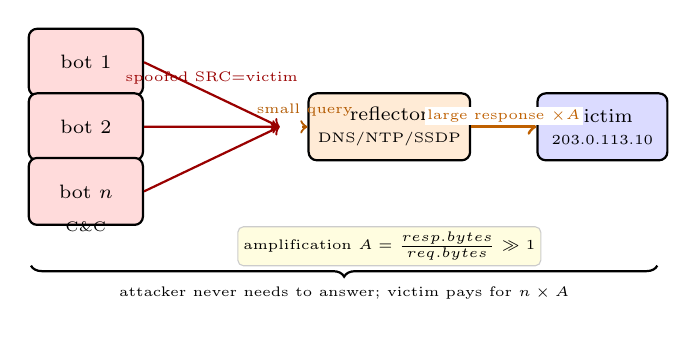
\begin{tikzpicture}[scale=0.82, every node/.style={font=\scriptsize},
  bot/.style={draw,thick,fill=red!14,rounded corners=3pt,minimum width=1.45cm,minimum height=0.85cm,align=center},
  amp/.style={draw,thick,fill=orange!16,rounded corners=3pt,minimum width=1.65cm,minimum height=0.85cm,align=center},
  vic/.style={draw,thick,fill=blue!14,rounded corners=3pt,minimum width=1.65cm,minimum height=0.85cm,align=center}]
\node[bot] (b1) at (0,2.0) {bot 1}; \node[bot] (b2) at (0,1.0) {bot 2}; \node[bot] (b3) at (0,0) {bot $n$}; \node[font=\tiny] at (0,-0.55) {C\&C};
\draw[->,thick,red!60!black] (b1.east) -- (3.0,1.0) node[midway,above,font=\tiny] {\tiny spoofed SRC=victim};
\draw[->,thick,red!60!black] (b2.east) -- (3.0,1.0); \draw[->,thick,red!60!black] (b3.east) -- (3.0,1.0);
\node[amp] (ref) at (4.7,1.0) {reflector\\\tiny DNS/NTP/SSDP};
\node[vic] (vic) at (8.0,1.0) {victim\\\tiny 203.0.113.10};
\draw[->,thick,orange!70!black] (3.35,1.0) -- (ref.west) node[midway,above,font=\tiny] {small query};
\draw[->,thick,orange!75!black,line width=1.1pt] (ref.east) -- (vic.west) node[midway,above,font=\tiny,fill=white,inner sep=1pt] {large response $\times A$};
\node[font=\tiny,fill=yellow!12,rounded corners=2pt,inner sep=2pt,draw=gray!40] at (4.7,-0.85) {amplification $A=\frac{\text{resp. bytes}}{\text{req. bytes}}\gg 1$};
\draw[decorate,decoration={brace,mirror,amplitude=4pt},thick] (-0.85,-1.15) -- (8.85,-1.15) node[midway,below=4pt,font=\tiny] {attacker never needs to answer; victim pays for $n\times A$};
\end{tikzpicture}}%
\caption{Amplification DDoS kill-chain. Bots send small spoofed queries; open reflectors reply with large responses to the victim. $A$ of $20$--$500\times$ is common with DNS/NTP.}
\label{fig:amplification}
\end{figure}

\begin{definition}[Amplification factor]\label{def:amp}
For a reflector $R$, $A_R = (\text{bytes in response})/(\text{bytes in request})$ as seen by $R$. The victim sees $n\cdot A_R$ times the attacker's upstream. Open DNS with ANY or DNSSEC validates $A\approx 30$--$60$; NTP monlist reached $>500\times$ before being disabled. Mitigation: close open reflectors and enforce ingress BCP38 anti-spoofing.
\end{definition}

Botnets provide $n$; reflectors provide $A$. Mirai (2016) showed how IoT defaults create $n\approx 600$k; a single open DNS population still numbers in the millions. BCP38 (ingress filtering) would kill spoofed sources, but deployment is incomplete, so the defender must assume $n$ and $A$ are both large.

\section{Protocol Exhaustion: The SYN Flood}\label{sec:synflood}
TCP's three-way handshake keeps state after the first SYN. A server with backlog $B$ (often 128--4096) allocates a transmission control block per half-open. A SYN flood sends SYNs from spoofed or bot IPs and never completes the handshake; the backlog fills, and legitimate SYNs are dropped with no answer.

\begin{figure}[h]\centering
\resizebox{\linewidth}{!}{%
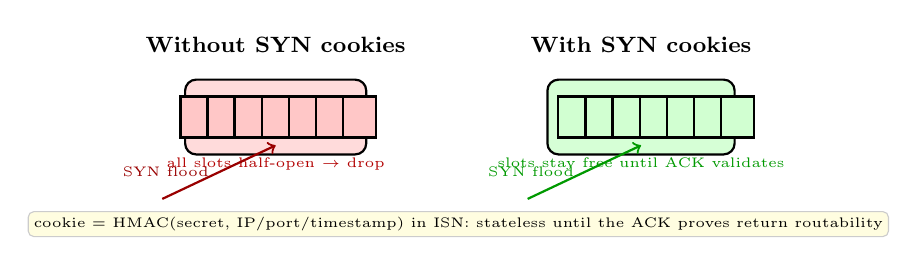
\begin{tikzpicture}[scale=0.80, every node/.style={font=\scriptsize},
  box/.style={draw,thick,rounded corners=4pt,minimum width=2.3cm,minimum height=0.95cm,align=center},
  slot/.style={draw,thick,minimum width=0.42cm,minimum height=0.52cm,inner sep=0pt}]
\node[font=\footnotesize\bfseries] at (2.0,3.0) {Without SYN cookies};
\node[box,fill=red!14] (q1) at (2.0,1.85) {backlog $B$ slots};
\foreach \x in {0.75,1.18,1.61,2.04,2.47,2.90,3.33} {\node[slot,fill=red!22] at (\x,1.85) {};}
\node[font=\tiny,red!70!black] at (2.0,1.10) {all slots half-open $\to$ drop};
\draw[->,thick,red!60!black] (0.2,0.55) -- (2.0,1.40) node[midway,left,font=\tiny] {SYN flood};
\node[font=\footnotesize\bfseries] at (7.8,3.0) {With SYN cookies};
\node[box,fill=green!16] (q2) at (7.8,1.85) {no per-SYN state\\\tiny cookie in ISN};
\foreach \x in {6.75,7.18,7.61,8.04,8.47,8.90,9.33} {\node[slot,fill=green!18] at (\x,1.85) {};}
\node[font=\tiny,green!60!black] at (7.8,1.10) {slots stay free until ACK validates};
\draw[->,thick,green!60!black] (6.0,0.55) -- (7.8,1.40) node[midway,left,font=\tiny] {SYN flood};
\node[font=\tiny,fill=yellow!12,rounded corners=2pt,inner sep=2pt,draw=gray!40] at (4.9,0.15) {cookie $=$ HMAC(secret, IP/port/timestamp) in ISN: stateless until the ACK proves return routability};
\end{tikzpicture}}%
\caption{SYN backlog exhaustion vs.\ SYN-cookie rescue. Cookies trade a cryptographic check for per-connection state and keep the queue available for legitimate clients.}
\label{fig:syncookie}
\end{figure}

\emph{SYN cookies} remove the trade: instead of storing state, the server encodes it into the initial sequence number $ISN = H(\text{secret}, \text{src/dst IP/port}, t) \Vert t \Vert MSS$. Only a final ACK that echoes a valid cookie recreates the connection. Cost: TCP options (window scaling, SACK) are limited during cookie mode, so Linux enables cookies only under pressure (\texttt{net.ipv4.tcp\_syncookies=1}).

Rate and SYN policing complement cookies: \texttt{nft limit} or XDP/eBPF drops excessive SYNs per source or per prefix before they reach the stack, but aggressive policing also drops legitimate bursts (e.g., a campus NAT behind one IP). The right balance is cookies as safety net plus a loose per-/24 policer that triggers only during flood.

\begin{lstlisting}[language=Python,caption={Lab-safe SYN flood with Scapy in an isolated netns (never run on production).},label={lst:synflood}]
from scapy.all import IP, TCP, send
dst = "10.0.5.10"   # lab victim in the same netns
for i in range(200):
    pkt = IP(dst=dst)/TCP(dport=80, flags="S", seq=1000+i, sport=40000+i)
    send(pkt, verbose=0)
# Observe on victim: ss -t -a | grep SYN-RECV ; dmesg | grep "possible SYN flood"
# Mitigate: echo 1 > /proc/sys/net/ipv4/tcp_syncookies ; sysctl net.ipv4.tcp_max_syn_backlog
\end{lstlisting}

\begin{lstlisting}[language=bash,caption={SYN policing before the stack: nftables and XDP intuition.},label={lst:syn-police}]
# nftables: rate-limit new SYNs, burst 40, then drop
nft add rule inet filter input tcp flags syn / syn,rst limit rate over 100/second burst 40 packets drop
# Check cookie mode is on and backlog counters
sysctl net.ipv4.tcp_syncookies
cat /proc/net/netstat | tr ' ' '\n' | grep -i syncookies
# XDP/eBPF sketch: drop SYNs exceeding per-/24 counter with a BPF map (see Ch.3 eBPF stub)
\end{lstlisting}

\section{Application Floods and Pulsing}\label{sec:appflood}
An attacker who cannot fill the pipe can still burn the server. A single HTTP GET may trigger a DB query, a template render, and a TLS handshake. At scale, legitimate-looking requests become a cost-asymmetry weapon: the attacker sends cheap requests, the server does expensive work. TLS renegotiation, regex backtracking (ReDoS), and large-range HTTP Range headers are classic amplifiers at layer~7.

Pulsing exploits time instead of size. A 10\,s burst at 10\,Gbps followed by 50\,s idle has an average that stays under a 5\,Gbps threshold, yet each burst fills shallow buffers and triggers retransmissions. Detection needs short windows (1--5\,s) plus a counter that remembers recent bursts. Carpet-bombing does the same in space: spreading traffic over many IPs in a /24 forces a prefix-wide filter that risks collateral damage.

Mitigation at L7 combines WAF signatures (block known expensive patterns), proof-of-work or CAPTCHA for suspicious clients, and autoscaling with a budget cap so scaling does not become a billing DoS. The cheapest fix is often to make the expensive endpoint cheaper: cache, paginate, and limit range headers.

% ============================================================

\begin{remark}[Why BCP38 is not enough]\label{rem:bcp38}
Ingress filtering (BCP38) would stop spoofed sources at the edge, but deployment is uneven: many access networks still forward packets with any source IP. ROV and SAV drafts push providers, yet an attacker needs only a few non-compliant ASes to launch an amplification flood. Defence must assume spoofing remains possible and combine edge filtering with reflector hygiene: disable open resolvers, turn off NTP monlist, and rate-limit SSDP/CHARGEN at the reflector itself.
\end{remark}

\begin{table}[h]\centering\small
\begin{tabular}{l l l l}
\toprule \textbf{Vector} & \textbf{Amplification $A$} & \textbf{Bandwidth at reflector} & \textbf{Hygiene fix} \\ \midrule
DNS ANY/DNSSEC & $30$--$60\times$ & open resolver, large TXT & RRL, close recursion \\
NTP monlist & $>500\times$ & monlist enabled & upgrade, disable monlist \\
SSDP & $20$--$30\times$ & UPnP on WAN & disable WAN UPnP \\
Memcached & $10\,000$--$50\,000\times$ & unauth UDP 11211 & firewall, auth \\ \bottomrule
\end{tabular}
\caption{Common reflectors ordered by amplification and the fix that removes them. Closing the reflector is cheaper than scrubbing its traffic forever.}
\label{tab:reflectors}
\end{table}

A defender's cost model is bytes $\times$ time $\times$ collateral. Dropping at the victim is free but the link is already full; scrubbing costs per clean Mbps but preserves the link; Anycast needs standing PoPs but amortises over all customers. Budget for clean capacity, not just filter rules.

\section{Scrubbing, Anycast, and the Playbook}\label{sec:scrub}
When the access link is saturated, filtering at the victim is already too late. Three escalations move the fight upstream.

\begin{figure}[h]\centering
\resizebox{\linewidth}{!}{%
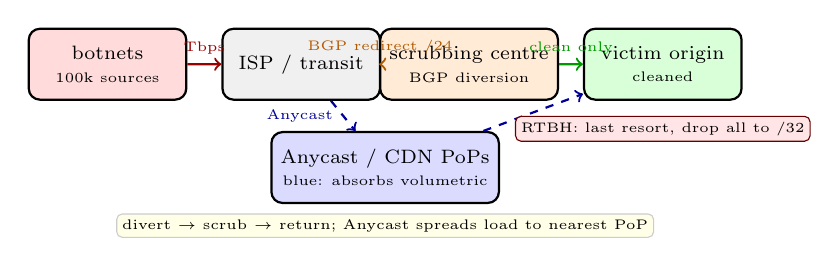
\begin{tikzpicture}[scale=0.82, every node/.style={font=\scriptsize},
  net/.style={draw,thick,rounded corners=4pt,minimum width=2.0cm,minimum height=0.90cm,align=center}]
\node[net,fill=red!14] (bot) at (0,1.65) {botnets\\\tiny 100k sources};
\node[net,fill=gray!12] (isp) at (3.0,1.65) {ISP / transit};
\node[net,fill=orange!16] (scrub) at (5.6,1.65) {scrubbing centre\\\tiny BGP diversion};
\node[net,fill=green!15] (vic) at (8.6,1.65) {victim origin\\\tiny cleaned};
\node[net,fill=blue!14] (any) at (4.3,0.05) {Anycast / CDN PoPs\\\tiny blue: absorbs volumetric};
\draw[->,thick,red!60!black] (bot) -- (isp) node[midway,above,font=\tiny] {Tbps};
\draw[->,thick,orange!70!black] (isp) -- (scrub) node[midway,above,font=\tiny] {BGP redirect /24};
\draw[->,thick,green!60!black] (scrub) -- (vic) node[midway,above,font=\tiny] {clean only};
\draw[->,thick,dashed,blue!60!black] (isp) -- (any) node[midway,left,font=\tiny] {Anycast};
\draw[->,thick,dashed,blue!60!black] (any) -- (vic);
\node[font=\tiny,fill=yellow!10,rounded corners=2pt,inner sep=2pt,draw=gray!40] at (4.3,-0.85) {divert $\to$ scrub $\to$ return; Anycast spreads load to nearest PoP};
\node[font=\tiny,fill=red!10,rounded corners=2pt,inner sep=2pt,draw=red!40!black] at (8.6,0.65) {RTBH: last resort, drop all to /32};
\end{tikzpicture}}%
\caption{Upstream defences. Volumetric traffic is diverted via BGP to a scrubbing centre or absorbed by Anycast/CDN; clean traffic is re-injected via GRE/MPLS. Remote-triggered blackholing is the emergency brake.}
\label{fig:scrubbing}
\end{figure}

\emph{Scrubbing centre:} BGP announces the victim /24 from the scrubber with a more specific or community-tagged route, diverts traffic via GRE, filters (SYN validation, amplification signature, flowspec), and returns clean traffic. \emph{Anycast/CDN:} the same IP is announced from many PoPs; each attacker is routed to the nearest PoP and the total is partitioned. \emph{Flowspec/RTBH:} BGP flowspec pushes 5-tuple filters to peers; remote-triggered blackholing drops all traffic to a /32 to save the rest of the network at the cost of the target.

Scrubbing adds latency (detour) and cost (clean bandwidth billed) but preserves availability; Anycast scales horizontally but only for stateless volumetric; RTBH is free and immediate but sacrifices the victim to protect neighbours. Choose by blast radius: RTBH for a single dispensable IP, scrubbing for a critical /24, Anycast as standing absorption for public web.

\vspace{0.2em}
\noindent\textbf{Playbook} (detect$\to$classify$\to$filter$\to$scale$\to$post-mortem):
\textit{Detect} via NetFlow/sFlow spikes and SYN-RECV counters; \textit{classify} as volumetric/protocol/app by ratio of bytes/PPS/flows; \textit{filter} nearest the source (BCP38 + flowspec) and locally (cookies, WAF); \textit{scale} by diverting to scrubber or Anycast; \textit{post-mortem} with a timeline, IoCs, and costed fixes. Every step has a pre-written runbook and a named owner. Test it with a tabletop before the real flood; the first time you run a playbook should not be during the incident.
Test the playbook without an attacker: inject a synthetic NetFlow spike, trigger the runbook, and time each handover. A playbook that has never been table-topped will fail its first real execution on a missing credential or a stale BGP community. Loop until clean, then post-mortem with timeline and owner.


% ============================================================
\section{Exercises}\label{sec:ch05-exercises}
\begin{enumerate}[label=E5.\arabic*, leftmargin=*, itemsep=0.6em]
    \item \textbf{Taxonomy.} Give one concrete attack for each of volumetric, protocol, and application DDoS. For each, state the bottleneck it exhausts and why filtering near the victim may already be too late.
    \item \textbf{Amplification arithmetic.} A DNS ANY response is 3\,000\,B for a 60\,B query ($A=50$). $500$ bots each send 2\,Mbps of queries via reflectors. What rate hits the victim? Propose two fixes that cut $A$ at the reflector rather than at the victim.
    \item \textbf{SYN flood lab.} In an isolated netns, use Listing~\ref{lst:synflood} against a lab VM with \texttt{tcp\_syncookies=0} and \texttt{=1}. Measure established vs.\ dropped legitimate connections with \texttt{ss -s} and \texttt{dmesg}. Explain the cookie's trade-off on TCP options.
    \item \textbf{Scrubbing decision.} A /24 hosts one critical API (needs 99.99\%) and one blog. Volumetric flood targets the blog's IP. Compare BGP RTBH (/32) vs.\ scrubbing diversion vs.\ Anycast absorption on blast radius, time to divert, and cost. Which do you choose?
    \item \textbf{Playbook tabletop.} A pulsing SYN flood (10\,s on, 50\,s off) evades a 60\,s-average rate limit. Write a detection rule using a 5\,s window plus SYN-cookie activation, and draft the post-mortem section that prevents recurrence.
\end{enumerate}

\begin{remark}[Operational note]\label{rem:opnote}
This design assumes continuous tuning, not a one-time deploy. Thresholds drift with traffic growth; retrain baselines monthly and after any architecture change. A threshold that was correct at 1\,Gbps is noise at 10\,Gbps.
Log retention is a cost decision: 30\,days of full NetFlow at 10\,Gbps sampled 1:100 is $\approx$2\,TB; justify it against the forensics window your IR team needs. Keep honeynet logs longer because they are tiny and high value.
Every automation (auto-block, auto-quarantine) needs a manual override and an audit trail. An auto-block that triggers on a CDN PoP will outage your own users; require a second signal (e.g., honeynet + NetFlow) before blocking a /24.
\end{remark}
Budget for clean capacity separately from filter rules: a 10\,Gbps scrubbing contract that is never tested is a hope, not a plan. Negotiate burst pricing and test diversion quarterly, including the return path via GRE and the BGP community that triggers it.
Measure collateral: a per-/24 policer that blocks a university NAT will drop hundreds of legitimate users for one attacker behind the same prefix. Prefer per-/32 plus reputation over per-prefix where flows allow, and log every block with its 5-tuple for appeal.
Application teams own L7 cost: add a cache header, paginate expensive queries, and enforce a max Range length. The cheapest DDoS mitigation is often a code change that makes one request ten times cheaper, documented in the post-mortem as a permanent fix.
Keep a public status page and a private war room. Volumetric floods are visible externally; a timely ``we are diverting via scrubbing, expect +20\,ms'' reduces support tickets and pressures the provider to meet its SLA.
Record every incident as a timeline: first NetFlow anomaly, first SYN-RECV spike, first WAF hit, diversion start, clean return, and customer impact. Cost the incident in clean bandwidth and engineering hours; that number funds the next mitigation.
Do not forget IPv6: many scrubbers and flowspec deployments still lag on v6. An attacker who cannot saturate v4 may try v6; ensure RPKI, BCP38, and SYN cookies are enabled on both stacks and that Anycast covers v6 as well.
The goal is graceful degradation, not perfect absorption. If the scrubber is overwhelmed, shed the lowest-value traffic first (blog, images) and protect the API with priority queuing. Document the shed order in advance so the on-call does not decide under fire.
Finally, close reflectors at the source: scan your own address space for open DNS, NTP, SSDP, and memcached and close them. You are both potential victim and unwitting amplifier; hygiene is a community defence.
Automate reflector hygiene with weekly scans: run \texttt{zmap} for UDP 53/123/1900 from a measurement net and notify owners of open reflectors. Community scanning reduces the amplifier population faster than any scrubber.
Separate infrastructure cost from attack cost: an attacker pays for bots and spoofed queries, the defender pays for clean bandwidth and on-call hours. Budget the incident in both, and show the cost of not closing reflectors.
Test scrubbing diversion with a benign prefix: announce a test /24 via the scrubber, measure latency via \texttt{mtr}, and verify return via GRE. Do this monthly so the BGP community and tunnel are not stale when needed.
Document the RTBH one-pager: which peer, which community, which /32, and who can authorize it. Under stress, an unpracticed RTBH will blackhole the wrong prefix and extend the outage.
Prefer BCP38 plus SAV at the edge: source-address validation is the only cure for spoofed amplification. Support MANRS and require upstream peers to filter, even if compliance is incremental.
For SYN floods, monitor retransmits: a legitimate client that retransmits SYN but never reaches ESTABLISHED is evidence of backlog fill, not client failure. Graph retransmits alongside SYN-RECV.
Application teams should own L7 budgets: each endpoint gets a cost tag (DB queries, external calls) and a latency SLO. An endpoint whose p95 exceeds 500\,ms under normal load is a DoS amplifier waiting to happen.
Do not autoscale without a ceiling: a 10\,Tbps flood that triggers autoscaling will become a 10\,Tbps bill. Cap scale and shed low-value traffic when cost exceeds a threshold; document the shed order.
Honeynet hits during a DDoS are not noise: an attacker who floods one prefix may probe another for a backdoor. Correlate volumetric spikes with honeynet probes in the same time window.
Post-mortem must include reflector data: which reflectors were abused, their ASes, and whether abuse reports were sent. Closing one reflector is more valuable than scrubbing its traffic ten times.
IPv6 is not exempt: many DDoS tools now support v6. Ensure the scrubber, flowspec, and Anycast cover your v6 prefix and that SYN cookies are enabled for v6 as well.
Keep a public runbook for customers: ``under DDoS, we will divert via scrubbing, expect +15\,ms, status at status.example.com''. Transparency reduces support load during the flood.
Energy and compliance matter: a scrubbing centre that diverts all traffic through another continent may breach data residency. Choose scrubber geography with legal, not just network, input.
Rehearse pulsing detection with synthetic bursts: inject 5\,s, 20\,Gbps bursts every 50\,s and verify the short-window detector fires. Long-average detectors will miss it; short-window plus burst counter will not.
Test scrubbing at L7 as well: a WAF rule that blocks the expensive ``search?q=*'' pattern during flood can cut CPU while the scrubber cuts bandwidth. Both are needed for app-layer floods.
Keep a darknet sensor in the same prefix as the critical API: any scan that hits the darknet before the API is a pre-attack signal, and its IoCs can be fed to flowspec before the flood peaks.
Coordinate with upstream: a single email to the transit with flowspec and RTBH communities is faster than any local filter when the link is already full. Pre-register the communities.
Budget the post-mortem: every incident should produce one permanent fix (close a reflector, add a cache, tune a WAF) and one detection improvement (new SIEM rule or shorter window). Without a fix, the next flood is the same flood.
Document the playbook owner and backup owner: an incident that starts when the primary is on a flight will fail if the backup does not know the BGP community or the scrubber portal login.
\section*{Chapter Notes}
DDoS taxonomy and reflector amplification follow Rossow (2014) and the classic DNS/NTP/SSDP studies; BCP38 ingress filtering is Ferguson--Senie (RFC~2827). SYN cookies are Bernstein--Schenk (1996) and Linux \texttt{tcp\_syncookies}; XDP/eBPF filtering is in the Cilium/eBPF docs. Scrubbing, flowspec (RFC~5575), RTBH (RFC~3882), and Anycast/CDN absorption are covered in NIST SP~800-189 and Arbor/WIT reports. The playbook mirrors SANS DDoS and Google SRE incident lifecycle.

% End of Chapter 5
